\documentclass[fontsize=11pt]{article}
\usepackage{amsmath}
\usepackage[utf8]{inputenc}
\usepackage[margin=0.75in]{geometry}
\usepackage[utf8]{inputenc}
\usepackage[T1]{fontenc}
\usepackage[american]{babel}
\usepackage{biblatex}
\usepackage{csquotes}

\usepackage{svg}

\begin{filecontents}{mla-withdabois.bib}


@online{epa, title={Greenhouse Gas Emissions from a Typical Passenger Vehicle}, url={https://www.epa.gov/greenvehicles/greenhouse-gas-emissions-typical-passenger-vehicle#:~:text=typical passenger vehicle?-,A typical passenger vehicle emits about 4.6 metric tons of,8,887 grams of CO2.}, journal={EPA}, publisher={Environmental Protection Agency}}

@misc{team, title={Keras documentation: The Sequential model}, url={https://keras.io/guides/sequential_model/}, journal={Keras}, author={Team, Keras}}

@misc{lamb_2019, title={How Does Carbon Dioxide Affect the Environment?}, url={https://sciencing.com/carbon-dioxide-affect-environment-8583965.html}, journal={Sciencing}, author={Lamb, Sheri}, year={2019}, month={Mar}}

@misc{liu_ciais, title={US Carbon monitor}, url={https://us.carbonmonitor.org/}, journal={Carbon monitor}, author={Liu, Zhu and Ciais, Philippe}}

@Article{Liu2020,
author={Liu, Zhu
and Ciais, Philippe
and Deng, Zhu
and Davis, Steven J.
and Zheng, Bo
and Wang, Yilong
and Cui, Duo
and Zhu, Biqing
and Dou, Xinyu
and Ke, Piyu
and Sun, Taochun
and Guo, Rui
and Zhong, Haiwang
and Boucher, Olivier
and Br{\'e}on, Fran{\c{c}}ois-Marie
and Lu, Chenxi
and Guo, Runtao
and Xue, Jinjun
and Boucher, Eulalie
and Tanaka, Katsumasa
and Chevallier, Fr{\'e}d{\'e}ric},
title={Carbon Monitor, a near-real-time daily dataset of global CO2 emission from fossil fuel and cement production},
journal={Scientific Data},
year={2020},
month={Nov},
day={09},
volume={7},
number={1},
pages={392},
abstract={We constructed a near-real-time daily CO2 emission dataset, the Carbon Monitor, to monitor the variations in CO2 emissions from fossil fuel combustion and cement production since January 1, 2019, at the national level, with near-global coverage on a daily basis and the potential to be frequently updated. Daily CO2 emissions are estimated from a diverse range of activity data, including the hourly to daily electrical power generation data of 31 countries, monthly production data and production indices of industry processes of 62 countries/regions, and daily mobility data and mobility indices for the ground transportation of 416 cities worldwide. Individual flight location data and monthly data were utilized for aviation and maritime transportation sector estimates. In addition, monthly fuel consumption data corrected for the daily air temperature of 206 countries were used to estimate the emissions from commercial and residential buildings. This Carbon Monitor dataset manifests the dynamic nature of CO2 emissions through daily, weekly and seasonal variations as influenced by workdays and holidays, as well as by the unfolding impacts of the COVID-19 pandemic. The Carbon Monitor near-real-time CO2 emission dataset shows a 8.8{\%} decline in CO2 emissions globally from January 1st to June 30th in 2020 when compared with the same period in 2019 and detects a regrowth of CO2 emissions by late April, which is mainly attributed to the recovery of economic activities in China and a partial easing of lockdowns in other countries. This daily updated CO2 emission dataset could offer a range of opportunities for related scientific research and policy making.},
issn={2052-4463},
doi={10.1038/s41597-020-00708-7},
url={https://doi.org/10.1038/s41597-020-00708-7}
}



\end{filecontents} % This is the end of the sample bibliography

\addbibresource{mla-withdabois.bib} % you would use your own bib file here

\title{Investigation Of Covid’s Impact On Carbon Emission Rates In the United States}
\author{Ahmed Khalf \and Rohan Mistry \and Eric Karpovits \and Shaffaan Bin Aamir}
\date{Tuesday, December 14, 2021}

\begin{document}
\maketitle

%\setcounter{section}{1}
\section{Problem Description and Research Question}

In our project, we want to explore the question, \textbf{how can we use models to predict whether COVID-19 decreased, increased, or had little effect on carbon emissions in the United States?} To understand this problem, the reader will need to know what the data is, the basic impacts of carbon emissions on the environment, and how the emissions are measured. We created 2 plots that help the reader understand the data. Also, a graphical user interface will allow anyone to understand the code without running any of the functions. The bar plot and line graph displays the emissions and emissions by state to be easily understood. The data measured carbon emissions from January 1, 2019, to September 30, 2021. They based carbon emissions on fossil fuel combustion and cement production. The carbon dioxide emissions are measured in metric tonnes, which is equivalent to 1000 kilograms. For reference, a single car produces about 4.6 metric tonnes of carbon dioxide per year \cite{epa}. Carbon dioxide has many negative effects on the environment. Since it is a greenhouse gas, it traps heat. This contributes to climate change and the destruction of the natural environment. Carbon emissions are caused by numerous sectors mainly ground transport, industries, international aviation, and power generation. The motive of choosing this as our research question is that COVID-19 impacted transportation, energy, industries, which all have a significant impact on carbon emissions. We want to go into detail and actually examine the effect COVID-19 had on carbon dioxide emissions by creating a model which uses data of carbon emissions prior to COVID-19 and predicts how carbon emissions would have looked like if COVID not occurred. The WHO declared COVID-19 as a pandemic on March 11, therefore, we will want to use our data to predict what would have happened from 2020-2021. Finally, we will compare this with actual data to understand to what extent there is a difference between them. To remove biases within the data, we want to normalize it and compare the normalized outputs with the non-normalized outputs to see whether it makes a difference in emissions. Ultimately, we will have a graph that shows the differences between the actual emissions vs. our predicted emissions to draw conclusions for our research question.


\section{Dataset Description}

The data set we will be using is from the Carbon Monitor. It was developed by a team publishing their paper and work for Nature, titled, “Near-real-time monitoring of global CO2 emissions reveals the effects of the COVID-19 pandemic”, whose intent was to create a platform where anyone can access data and learn about the impact of fossil fuels and cement production on climate change ~\cite{liu_ciais}. The Carbon Monitor is an international data set that provides daily updated estimates of carbon dioxide emissions. The data is stored in a CSV file and contains daily carbon emissions in metric tons separated into several key emission sectors. The categories are the power sector (39\% of total emissions), industrial production (28\%), ground transport (19\%), air transport (3\%), ship transport (2\%), and residential consumption (10\%). In our project, we will want to sum up these sectors because we are looking for an overall trend in emissions rather than per sector. Carbon emissions are measured from January 1, 2020, to September 31, 2021. The uncertainty of the data set of global carbon emissions from fossil fuel burning and cement production varies between ± 6\% and ± 10\% (±2\(\sigma\))) \cite{Liu2020}. This is because the uncertainties are introduced by errors and inconsistencies in the reported figures from different sources that Carbon Monitor uses. There are five columns in the data: state, date, sector, value, and timestamp. We will exclude the last timestamp column. The reason we excluded the timestamp is because the second column already provides a date which we can convert to a datetime.date for use in code. 

\section{Computational Overview}

First, we will discuss our data.py file where we handle the data related computations of our project. We created the CarbonMetric data class as an abstraction for a row in our data. It has 4 main attributes, the state in which the carbon emission was recorded, the date as a datetime.date, a value for the emissions for that day in metric tonnes, and its specific sector which we set as an optional attribute. Next, our DataManager class is a class that is responsible for a majority of computations on the data. Its metric attribute stores a list of CarbonMetric, which is created when we use the load\_data() function which uses the native python csv module. The filter method is responsible for filtering the metrics list in place. It contains optional arguments for each parameter in carbon metrics. This allows us to filter the data for whichever metric we prefer. The normalize\_data() uses a mathematical formula that allows us to transform all the values of carbon metrics to numbers between 0 and 1 which can be helpful for removing biases in the output of our model. The sum\_of\_total\_emissions() method iterates through each day and accumulates the carbon emissions for a given state. One important aspect to notice is that the class methods for the DataManager class all mutate the self.metrics list. However, sometimes we want the original data to remain intact. Hence why we created a copy function, which returns a new DataManager.
In train.py, we used Keras to create a machine learning model that uses the LSTM architecture. The LSTM stands for Long Short Term Memory, and it is a type of recurrent neural network that is great at reading and predicting sequential data. First, we need to prepare the training data that will be used to train the model. Inside the prepare\_training\_data() function, we use the functions from data.py to read and filter the carbon metrics from the beginning of January 1, 2019, to February 11, 2020. Then we create two lists x\_train which is the input to the model, and y\_train which is the expected output.

\begin{center}
\vspace*{-2.25cm}
\includesvg[width=0.7\columnwidth]{xytrain.svg}
\vspace*{-4.75cm}
\end{center}

Furthermore, since the LSTM only accepts three dimensional input, further processing must be made in the reshape\_x\_data() function.

\begin{center}
\vspace*{-2.25cm}
\includesvg[width=0.7\columnwidth]{reshapex.svg}
\vspace*{-3.25cm}
\end{center}

Finally, using the Keras sequential API docs, we were able to create the model and train it \cite{team}. We trained two versions of the model. One that uses normalized data, while the other uses unnormalized data. After training the model with mapped data, we use the model to predict what would have happened to carbon emissions if COVID-19 did not occur.

In plot.py we used plotly to display the main parts of our data and the results from our prediction model. To better understand our data we created a line graph and bar chart. The line graph displays the data that was fed into the prediction model which is daily emissions for 2019. The bar chart helps display each state with its total emissions for 2019. We created the day\_to\_index\_mapping() and index\_to\_day\_list() functions to help plot and interpret the x-axis of our line graphs. The slope\_secant() function calculates the rate of change of emissions between 2 days. To use the slope formula we needed to map datetime.date values to integers starting at 0, this is why we used the day\_to\_index mapping. Our first main line graph displays the actual United States carbon emissions from 2020-2021 vs. our model’s prediction for emission. Our model outputs only the carbon values and does not have a date associated with it. To increase the accuracy of our model, the predictions begin on February 12, 2020 and end August 31, 2021. We use our index to day list to map all the values to dates, so our first prediction value gets mapped to February 12, 2020. Our second main line graph displays the difference between our model’s prediction. This allows us to visualize Covid’s impact on emissions and how low or drastic these differences are.

In ui.py, we used the Tkinter module to display our Python interface to a graphical user interface. We have built a user interface class in which we initialised buttons using the button class that comes built in Tkinter. We also use some of the options for this widget, such as: text, font, and orient. Each of these help us to format our button widgets. Each button widget is also assigned a command, which is to call a specific function from plot.py. For example, ‘Button1’ calls the ‘bar\_chart()’ function from plot.py. Our buttons were labelled with the name of the graphs and whenever the user clicks the button, the graph will open on their default browser.


\section{Instructions for obtaining data sets and running the program}

First, ensure all packages in requirements.py are installed.

Second, for your convenience, we have created an automatic system that downloads all required files with proper naming in the current directory. All you need to do is run the main.py file and both the data sets and pre-trained models will be downloaded automatically.

Lastly, when you run the main.py file, apart from downloading the data sets and models, you should expect to see a Tkinter window. When you click on one of the buttons in the Tkinter window, you should expect a browser tab to open which will contain the Plotly plot.

\begin{center}
    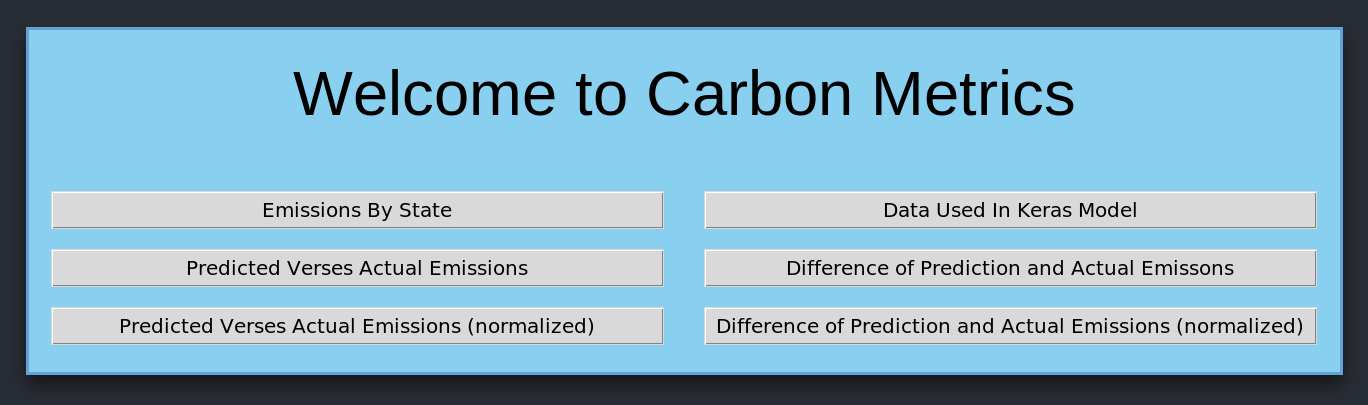
\includegraphics[scale=0.5]{app.png}
\end{center}

In case something goes wrong, here are links to the data sets automatically downloaded by main.py:

\renewcommand{\arraystretch}{1.5}
\begin{tabular}{ p{7cm} p{7cm} }
 carbonmonitor-us\_datas\_2021-11-04.csv & \url{https://drive.google.com/uc?id=1ZC_qrjWnTTt61e628Ejh-bBLh6CRdnq_} \\ 
 model.keras & \url{https://drive.google.com/uc?id=1Hqgdfd8S2i-aBpdseV9h1ByjArJywEA3} \\  
 normalized\_data\_model.keras & \url{https://drive.google.com/uc?id=1vodjV37FH3r7NfnMeYilteKwzYFZGPT8}    
\end{tabular}

\textit{Note to TA: Everyday, the carbon monitor database gets updated. Which is why we uploaded the database to Google Drive to freeze the data for reproducibility.}


\section{Changes since proposal}

Our final submission is slightly different from our proposal as we added more features and implemented TA feedback. Based on group discussion, we came to the consensus that a user interface is necessary to display all of our work in an elegant way without having to manually run functions in the python console. This simplifies the debugging process as we know that if our plotly plots work, then all of our data.py and train.py functions used in the corresponding plot functions work smoothly. Our group implemented all the feedback from the TA as it was helpful to answering our research question. As suggested, we trained the mathematical model with both normalized and unnormalized (regular) data to see whether there were any differences in the predictions. Furthermore, we made a line graph that displays the difference in emissions between our model’s predictions and the actual data as suggested by the TA.

\section{Program results, discussion, and analysis}

As a general trend, we saw that our unnormalized model overpredicts the emissions by around 0.4 metric tonnes of carbon. This means that if COVID had not occurred, there would have been a slight continued rise in emissions and that COVID generally slightly decreased emissions. However, for our normalized model, we saw a trend of under predictions by around -0.35 metric tonnes. This means that COVID only slightly increased daily emissions. Ultimately the differences were quite small so we can conclude that overall, COVID-19 did not have a major impact on the rate of carbon emissions in the United States. In the year 2019, the rate of increase of emissions was about 0.003 metric tonnes a day. It seems like a small value, but in the course of a year the emissions accumulate. The sharpest decrease was from January 31, 2019 to February 3, 2019 (a rate of about 2.1 metric tonnes per day) and the remainder of the year fluctuates between 13-14 metric tonnes per day. From February 12, 2020 to August 31, 2021, our normalized model predicted -0.0027 metric tonnes per day, unnormalized predicted -0.0026 metric tonnes per day, and the actual rate was about -0.0031 metric tonnes per day. This may seem surprising to see little difference, but if we investigate further into specific month ranges, we can understand why our models were accurate in showing a small change. The actual emissions from February 21, 2020 to April 15, 2020 decreased at a rate of -0.97 metric tonnes a day. Both our normalized and unnormalized models overpredict in this interval by about 1 metric tonne a day. This further shows that without COVID carbon emissions would have been more steady (increasing and decreasing wise). But, during COVID it had a sharp decrease during the initial lockdown periods. After life began going “back to normal” the emissions gradually began to increase back to where it normally was.  
In order to come up with the data and conclusions presented in the above paragraph, we used several plots that showcase the result of our computations. The one day predictions and actual values for the unnormalized model are shown below:

\begin{center}
    \includegraphics[scale=0.325]{image1.png}
\end{center}

Furthermore, the difference between the predicted value and the actual values for the unnormalized model is shown below:

\begin{center}
    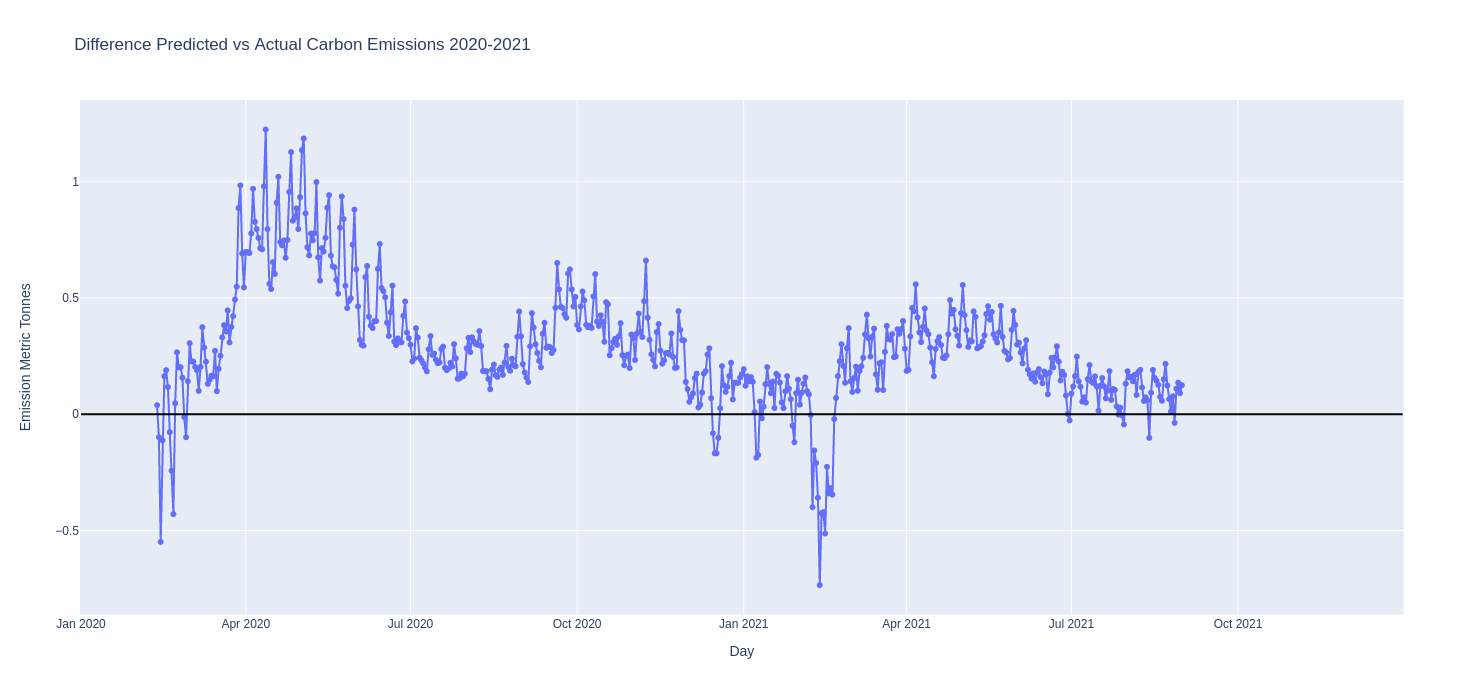
\includegraphics[scale=0.325]{image4.png}
\end{center}

Likewise, for the normalized model:

\begin{center}
    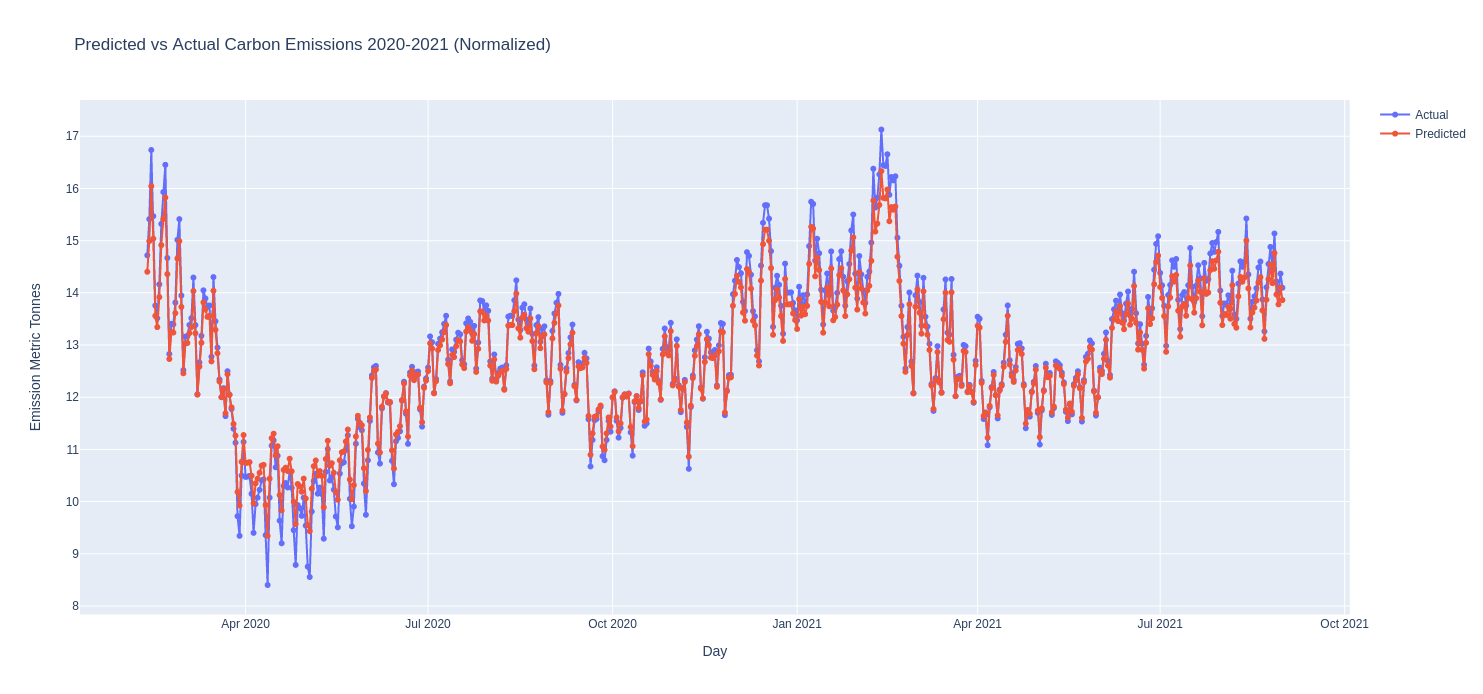
\includegraphics[scale=0.325]{image5.png}
\end{center}
\begin{center}
    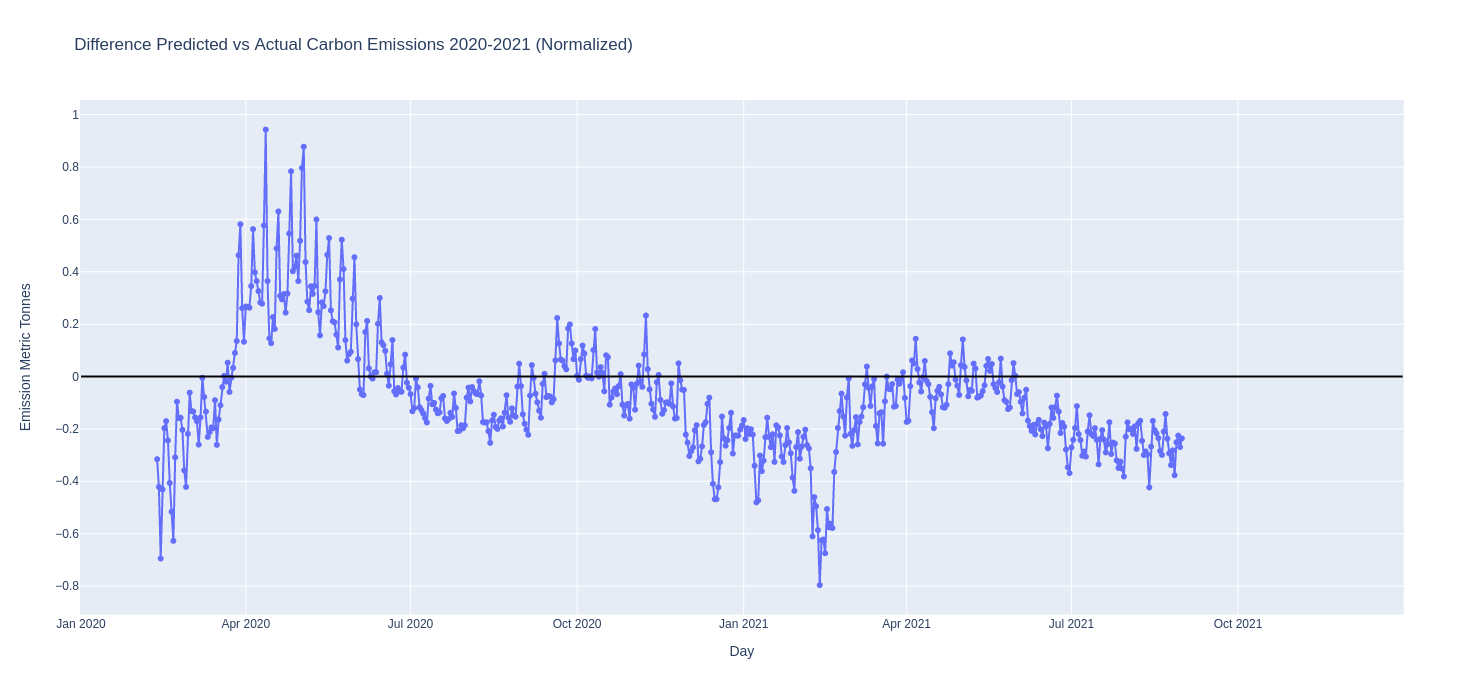
\includegraphics[scale=0.325]{image2.png}
\end{center}


There were some limitations in our data. We were only limited to 6 sectors of where carbon was emitted, this limits how much detailed analysis we can do on these. Also, there could be biases in the data as some types of emissions are grouped into one sector and some sectors are completely left out of the data. There was also a small percentage of uncertainty in our data. This may have slightly skewed our predictions as it was difficult to create a clear solution on how we could remove uncertainty. We can take multiple steps to further explore COVID’s impact on carbon emissions. We can do in-depth analysis on the change in emissions between sectors. From our model, we saw that COVID did not have a large impact. Therefore, we can create plots for each sector to see which sectors had increases and decreases in emissions which balanced out the overall emissions. Another limitation of our model is that it can only predict carbon value one day in advance. Therefore, in future explorations, we can generalise the model to predict n days ahead. 



\nocite{lamb_2019}

\printbibliography

% NOTE: LaTeX does have a built-in way of generating references automatically,
% but it's a bit tricky to use so we STRONGLY recommend writing your references
% manually, using a standard academic format like APA or MLA.
% (E.g., https://owl.purdue.edu/owl/research_and_citation/apa_style/apa_formatting_and_style_guide/general_format.html)

\end{document}
